\documentclass[letterpaper, 10pt,titlepage]{article}

\usepackage[utf8]{inputenc}
\usepackage [english]{babel}
\usepackage [autostyle, english = american]{csquotes}
\usepackage{graphicx}                                        
\usepackage{amssymb}                                         
\usepackage{amsmath}                                         
\usepackage{amsthm}                                          
\usepackage{alltt}                                           
\usepackage{float}
\usepackage{url}
\newcommand\tab[1][1cm]{\hspace*{#1}}
\setlength{\parindent}{0em}
\setlength{\parskip}{1em}
\usepackage{pst-gantt}
\usepackage[letterpaper, margin=0.75in]{geometry}
\usepackage{balance}
\usepackage[TABBOTCAP, tight]{subfigure}
\usepackage{enumitem}
\usepackage{pstricks, pst-node}
\usepackage{hyperref}
\hypersetup{
  colorlinks = true,
  linkcolor  = black
}
\usepackage{listings}
\usepackage{color}
 
\definecolor{codegreen}{rgb}{0,0.6,0}
\definecolor{codegray}{rgb}{0.5,0.5,0.5}
\definecolor{codepurple}{rgb}{0.58,0,0.82}
\definecolor{backcolour}{rgb}{0.95,0.95,0.92}
 
\lstdefinestyle{mystyle}{
    backgroundcolor=\color{backcolour},   
    commentstyle=\color{codegreen},
    keywordstyle=\color{magenta},
    numberstyle=\tiny\color{codegray},
    stringstyle=\color{codepurple},
    basicstyle=\footnotesize,
    breakatwhitespace=false,         
    breaklines=true,                 
    captionpos=b,                    
    keepspaces=true,                 
    numbers=left,                    
    numbersep=5pt,                  
    showspaces=false,                
    showstringspaces=false,
    showtabs=false,                  
    tabsize=2
}
 
\lstset{style=mystyle}
\usepackage{minted}




\setcounter{secnumdepth}{4}
\def\name{Jiawei Liu}

\hypersetup{
  colorlinks = true,
  urlcolor = black,
  pdfauthor = {\name},
  pdfkeywords = {Problem Statement},
  pdftitle = {Capstone Project},
  pdfsubject = {Capstone Project},
  pdfpagemode = UseNone
}



\begin{document}

\begin{titlepage}
\begin{center}
    \Huge
    \textbf{Technology Review Document}\\
    \textbf{Capstone Project}\\
    \vspace{1.0cm}
    \large
    Developers: Charles Henninger, Duncan Millard, Jiawei Liu\\
    Sponsor: Nancy Hildebrandt\\
    \vspace{1.5cm}
    \large
    Instructor: D. Kevin McGrath\\

    \large
    CS 461, Fall 2016, Oregon State University\\    

    \vspace{3.2cm}

    \large
    \underline{Abstract}\\
    \vspace{0.3cm}
    \end{center}
    \large

    \tab our new abstract should here XXXXXXXXXXXX
    
    \vspace{0.8cm}
    \vfill
    
\begin{center}    
    Nov 14, 2016

\end{center}
\end{titlepage}


\tableofcontents
\newpage



\section{Introduction}
\subsection{Team number and project name}
We are group \#43, and project name is Santiam Wagon Trail Mobile App.


\subsection{Team members and role in the project}
Jiawei Liu: iOS UI Design and Functionality, Web Control Panel UI, and iOS Remote API Interactions \\
Charles Henninger: Android UI Design and Functionality, Map Rendering, Android Remote API Interactions\\
Duncan Millard: Web Control Panel functionality, Inter-App framework

\vspace{0.3cm}




\section{Jiawei Liu's Section}

\subsection{iOS UI}
Since the project required to design a mobile app on iOS platform. Therefore, the usability is an important part of the project. In iOS user interface design section, the problems are designing and implementing the UI for selecting content packages, downloading and removing them, as well as basics for tour layout. For solving these problems, there are three technologies are effectual, which are mobile web pages, Xcode and OpenGL ES.


\textit{Solution A:} Mobile Web Page\\
A web page is a page that displays on web browsers via an internet connection. The mobile web page is a kind of webpage that optimized for mobile devices such as smart phones and tablets. The purpose of using a mobile web page is displayed the map on screen, allow user select and download content packages and provide the tour information.


A high-caliber mobile web page relies on various technologies such as HTML, Cascading Style Sheets (CSS), JavaScript and PHP. In general, HTML is the standard markup language employed to create web pages and its elements form the building blocks of all websites [1]. HTML can only serve as a basic web page. CSS and JavaScript are the necessary technologies for beautify and add more functions in the web page. If the web page uses database to hold website data, PHP is an efficient technology to connect and modify the database. 


Nowadays, our life is flooded with web pages. For example, Facebook, one of the most popular social website; Google Maps, a popular map website; YouTube, a famous video website. These websites are make-up of HTML, CSS, JavaScript and PHP. In addition, most websites also provide mobile version web page to bring better user experience with mobile devices. 


\textit{Solution B:} Using Xcode with Swift\\
Xcode is an integrated development environment (IDE) that developed by Apple. Developers can use Xcode to develop both iOS and macOS applications. The purpose of using Xcode is designing and implementing the UI by a tool or a IDE, Due to the high integration of Xcode, this can bring some convenient and save our time to build the development environment.  


For using Xcode with swift, it is necessary in order to get acquainted with Xcode. As Figure 1 show, Xcode has the object library on the right side, and allow developers to drag an object from the library to the application. There are not that many techniques in the UI design section, it basically selects the object from the library and drags it to the design area. It is simple and visible.

\begin{figure}[ht]
    \centering
    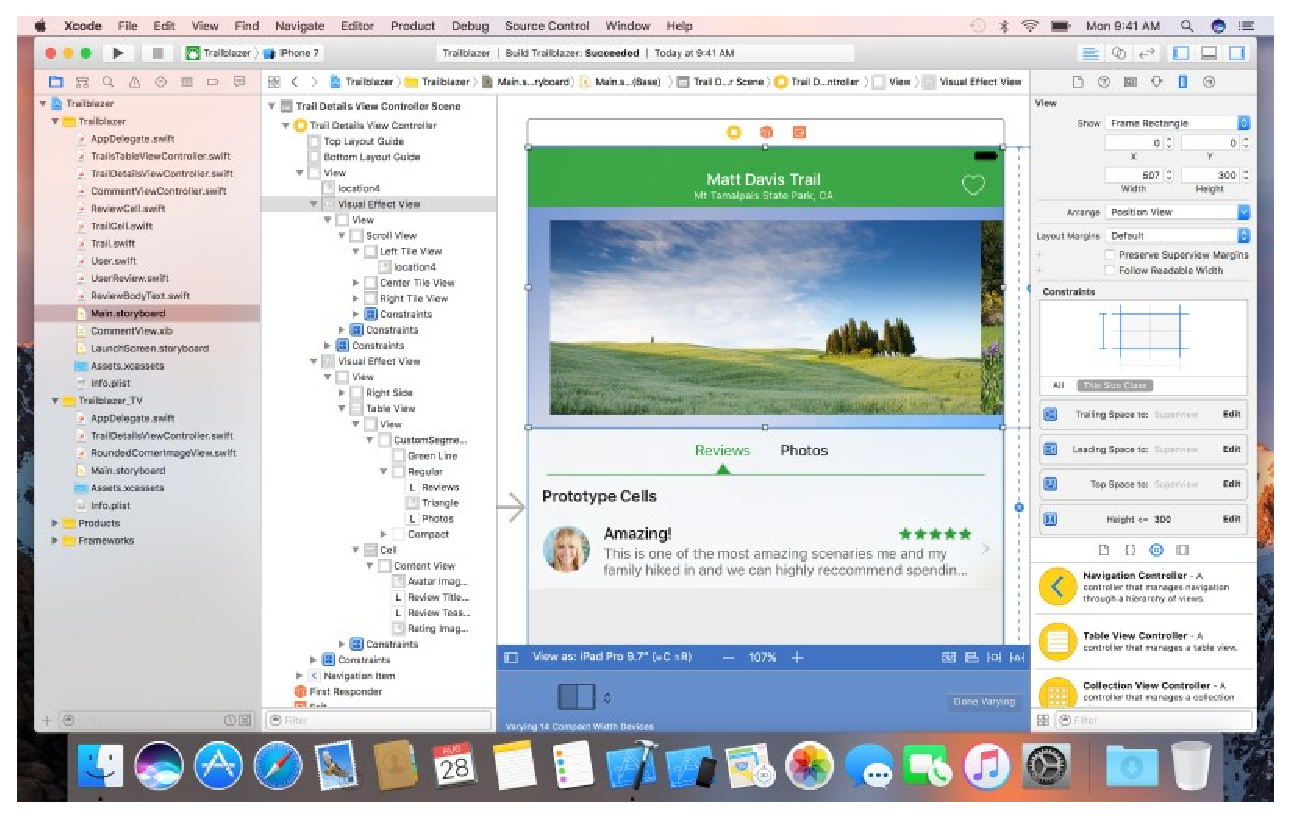
\includegraphics[width=0.9\textwidth]{j1}
    \caption{Xcode Interface [6]}
    \label{jiawei1}
\end{figure}

Xcode is the official IDE for developing iOS application, and is offered for free. Therefore, most iOS applications are developed by Xcode. For example, Safari, eBay, Expedia, etc.


\textit{Solution C:} OpenGL ES\\
OpenGL ES is a royalty-free, cross-platform API for full-function 2D and 3D graphics on embedded systems - including consoles, phones, appliances and vehicles [2]. Therefore, OpenGL ES is the third option to design the UI for provide tour information, view the map and interact with content packages. 


OpenGL is the core technology used for 2D and 3D graph. OpenGL ES is a simplified version of OpenGL that eliminates redundant functionality to provide a library that is both easier to learn and easier to implement in mobile graphics hardware [3]. Therefore, OpenGL ES is an efficient development tool to design iOS application UI. 


Most of iOS games are developed by OpenGL. For example, Flappy Brid can be developed by OpenGL ES easily. In addition, currently most iOS games are developed by OpenGL ES.


In conclusion, we are planning on going with our second solution, Xcode. Because we are going to write an iOS application, not a 2D or 3D game. Therefore, OpenGL is not the best solution for us. Our application also requires to use without an internet connection. Hence, the mobile web page is not fit in this situation. Xcode is the official IDE that provided by Apple. It includes a suite of development tools for iOS, macOS, WatchOS and tvOS. Due to high integration of Xcode, developer can develop software with minimal troubles. Even Xcode is offered for free, it only available on macOS. Two of our team members are using windows laptops. Thus, they need to set the virtual machine to access Xcode.


\subsection{Web Control Panel UI}
What has to be accomplished in this part of the solution is designing and implementing the tour creation. We need to design a website to allow administrators such as our client, Nancy to setup for map frame, click to add waypoints, click waypoints to add texts and videos. In order to control resource on the web, we need to design a dynamic website with a clear UI. Therefore, there are multiple methods that we can use for creating web control panel UI.


\textit{Solution A:} Bootstrap\\
Bootstrap is the most popular HTML, CSS, and JavaScript framework for developing responsive, mobile-first web sites [4]. In addition, Bootstrap is offered for free. Everybody can download and use it. The purpose of using Bootstrap is creating a dynamic website as the web control panel for our client to control online texts and videos resources. 


In general, syntax of Bootstrap is similar with HTML, which mentioned on “Mobile Web Page” section. However, Bootstrap is more powerful than HTML because it provided more functions such as preprocessors and universal framework. In addition, as Figure 2 shows, there are abundant themes available for free. We can apply these themes to create the website with an aesthetically pleasing UI. 

\begin{figure}[ht]
    \centering
    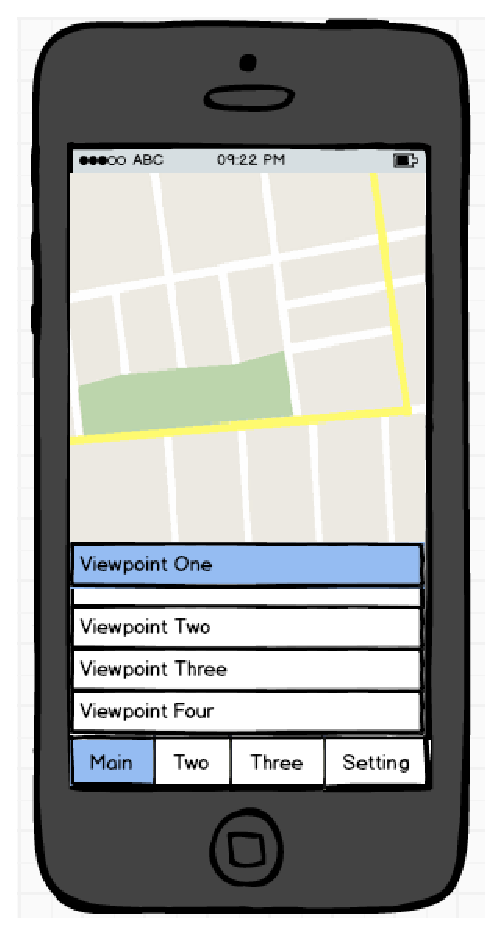
\includegraphics[width=0.9\textwidth]{j2}
    \caption{Free Bootstrap Templates [7]}
    \label{jiawei2}
\end{figure}

As the most popular framework for developing websites, there are a number of websites are using Bootstrap, such as NBA.com, Walmart, gliffy, etc. 


\textit{Solution B:} JavaScript\\
JavaScript is the programming language of HTML, and can be considered as a functional extension of HTML. JavaScript’s syntax is obvious and easy to learn. JavaScript can modify the web page’s layout such as HTML content, attributes and CSS. JavaScript’s functions are based on HTML and CSS, but JavaScript is a separate and high-level programming language. JavaScript also provided two useful features, which are AJAX and JSON. Both of them are helpful for our project. JavaScript is popular. There are some websites are using JavaScript: MapsTD, The Local Palette, tota11y, etc.


\textit{Solution C:} jQuery\\
jQuery is a library of JavaScript. The purpose of using jQuery is it easy to learn and apply in the web page. The jQuery library contains these features, which are HTML/DOM manipulation, CSS manipulation, HTML event methods, Effects and animations, AJAX and Utilities [5]. With jQuery, developers can write less code to achieve the same goal on web pages. 


Since jQuery is a JavaScript library and has many features of HTML, it based on JavaScript, HTML and CSS. We can consider jQuery as a highly integrated development tool to simplify web development process.


jQuery is a necessary technology for developing dynamic web pages. Therefore, a lot of famous websites used jQuery, such as Google Maps, Google Doc, Netflix, etc. 


In conclusion, our group is going to use both Bootstrap and jQuery due to design a high-quality dynamic website as the web control panel. JavaScript is a satisfactory technology. However, Bootstrap presents a wide range of convenient because of the highly-integration and better visual effect. jQuery simplifies JavaScript programming greatly. Therefore, we choose to utilize both Bootstrap and jQuery to design our web control panel.


\subsection{Remote API Interactions}
In this section, we are going to provide a solution that allows users download content packages to their iOS devices. Users also permit to see all available content packages and select the package that they wish to download. After users choose the package, the application start to download the package by making an API call to the web server. To achieve this goal, we have three technologies available, which are WKWebView, NSURLConnection and download from a phone browser.


\textit{Solution A:} WKWebView\\
WKWebView is a class of iOS to interactive web content, such as for an in-app browser [8]. The purpose of using WKWebView object in our application is interactive with our server and load content package list for users. There is a symbol in WKWebView called loading content. With this symbol, we are able to set the webpage contents and base URL for users, then the user can select and download the package. Here is an example about creating a WKWebView programmatically [8].

\begin{minted}{swift}
import UIKit
import WebKit
class ViewController: UIViewController, WKUIDelegate {
    
    var webView: WKWebView!
    
    override func loadView() {
        let webConfiguration = WKWebViewConfiguration()
        webView = WKWebView(frame: .zero, configuration: webConfiguration)
        webView.uiDelegate = self
        view = webView
    }
    override func viewDidLoad() {
        super.viewDidLoad()
        
        let myURL = URL(string: "https://www.apple.com")
        let myRequest = URLRequest(url: myURL!)
        webView.load(myRequest)
    }}
\end{minted}

WKWebView was starting at iOS 8. It is based on iOS operating system. Besides,  most iOS web browsers and in-app browsers are using WKWebView. For example, Safari and Twitter’s in-app browser. WKWebView is popular and necessary for iOS development.


\textit{Solution B:} NSURLConnection \\
NSURLConnection is similar with WKWebView. It is also a class iOS. A NSURLConnection object lets you load the contents of a URL by providing a URL request object [9]. Therefore, the purpose of using NSURLConnection is loading content packages from the web server by a URL request. 


As a class of iOS, it is built on iOS operating system, and has it own syntax. Most iOS applications are using NSURLConnection to connect to server and load packages. For example, some huge iOS games are required download data packages to the device. These games used NSURLConnection technology. And then, this situation is analogous with downloading content packages to iOS devices. 


\textit{Solution C:} download from phone browser \\
Since we have a web control panel for administrators, we can create a web page for users, and users can use phone browser such as Safari to view and download to phone storage. The purpose of using download from browsers is it is easy to implement and understand how this process works.


Downloading directly is popular in Windows and Android. For example, users download a mp3 file from the internet, and use music software to play this mp3 file. This process can also be implemented in iOS. Downloading directly is relying on many internet technologies such as Http, ftp, web pages, etc. 


In conclusion, we are going to use NSURLConnection technics to download content packages from the web server. For display and select the available content packages, we will use WKWebView to display the available package data from our server. The reason that we don’t choose downloading directly is iOS has strict limitation on file operating. In addition, there is not any file explorer on iOS. This will bring a lot of trouble for users. Therefore, we choose the native iOS API, WKWebView and NSURLConnection to accomplish our project.

\vspace{0.5cm}


\section{Charles Henninger's Section}
\subsection{Map Rendering}
What needs to be accomplished in this part of the solution is making a map visible and capable of interaction with the user. We will need to display a relevant map of the tour area, capable of zooming, refocusing on the location of the user, and displaying waypoints on the map that contain relevant information about the area, including videos and text files. In order to get quality offline map tiles that we can use in our application, we have decided to use libraries connected to OpenStreetMaps, a project that provides free geographic data for use in rendering maps. OpenStreetMaps has many libraries that may provide us the means to render maps offline.


While there are many libraries that use OpenStreetMap data, we will only be using one. The first option is a library called LibosmScout. LibosmScout is a simple client side library commonly used in smaller applications that need to render map tiles using OpenStreetMaps data offline. LibosmScout offers offline rendering of map tiles in a simple and easy to use library, as well as some minor features for drawing and editing a map offline, which could be valuable for this projec. LibosmScout is compatible with both IOS and Android platforms, and is written in C++ and Java. LibosmScout is a relatively new library, written under an LGPL license and maintained by a single developer. LibosmScout’s codebase is often changed and updated, which brings into question it’s reliability in the long term. LibosmScout seems to meet the bare minimum for what we need to do in rendering an offline map that the user can interact with, but it’s volatile codebase might make it too unreliable to use in our solution. 


Our second option is a suite of open-source libraries made by Mapbox used for rendering and navigating maps based on OpenStreetMap’s data. Using the SDK libraries provided in the Mapbox GL suite for both Android and IOS, we will easily be able to render maps offline at a commercial quality level. These libraries have a target language of Java for the Android SDK and Swift for the IOS SDK. Mapbox GL has a well maintained codebase that seems stable and professional, and is offered for free. 


The last option that we researched was a rendering service called Cartotype. This service is a high quality rendering service that works with online or local map tiles. The functionality is very similar to the Mapbox suite of libraries, although at a slightly higher quality. Cartotype is under a proprietary license, and will cost an undisclosed amount to use. 


At this point in time, we are planning on going with our second option, Mapbox GL, for implementation on both the IOS and Android platform. Due to the volatility of LibosmScout’s codebase, and the cost that would be required to use Cartotype, neither are considered to be a viable option for this solution. Mapbox GL is a free service that offers high quality rendering and mapping features offline, and brings with it many useful extra features such as custom waypoint and path editing.

\subsection{Android UI}
This piece of our solution will be the UI of the mobile app on the Android platform. We plan to conform to the Android UI guidelines for the layout of most of the UI. The technology we could use here, i.e. the main language used to create the UI, ranges from XML to SDL or Java. SDL, while great for animations and high end graphical features, is too complicated compared to the other two options, especially because it wouldn't help us all that much. Using Java for the UI would be slower, and would only benefit us if we needed tight control of the UI, which we don’t. 


The decision to use XML for our UI on our Android platform didn’t take much thought. XML is simpler, cleaner, and faster than other options like Java or SDL. 

\subsection{Remote API Interactions}
This piece of our solution involves how we will download our content package files from our server onto the mobile device. Users will view available content packs in app and select which content packs that they want to download. Once a user confirms a download, the mobile app will make an API call to our web server and begin downloading the file. There are multiple methods that we can use to initiate and facilitate the download, both native and non-native to the Android platform. 


Our first option, Retrofit, is a networking library that can facilitate downloading files from an online source. Retrofit is very easy to implement, and is faster than any of the other options that we looked at for this piece of our solution. Retrofit uses standard methods, which is why it is so easy to work with, but doesn’t have the capability for custom methods of caching and retrying. Unfortunately, Retrofit is geared towards smaller files than we will be working with for this application. 


Our next option, Volley, is very similar to Retrofit. Volley is another networking library used to facilitate downloading files on an android platform, and offers much more customizability in how it handles caching and retries compared to Retrofit. While slightly slower, Volley could potentially give us more control in the downloading process. Like Retrofit, Volley is meant for slightly smaller files than we will be downloading in this app.


Our last option is the native networking method for Android, the DownloadManager service. This service comes with many build in features, such as notifications for completed downloads, that would have to be manually added with Volley and Retrofit. DownloadManager is meant for larger files that require long running downloads. While Volley and Retrofit do provide more control over the downloading process compared to DownloadManager, more control simply isn’t necessary for this application. 


Implementing our application with either Volley or Retrofit would require more work and troubleshooting compared to using DownloadManager, and wouldn’t provide us any extra functionality for the app. For this reason, DownloadManager will be the service that we use for downloading files on the Android platform. 

\vspace{0.5cm}

\section{Duncan Millard's Section}
\subsection{Web Server Configuration}
When setting up any new project, one of the most critical segments is to determine what will the underlying architecture be for the current development and future release. This product solution is a three pieced tool, with a singular web server and two flavors of mobile application. The primary web server, referred internally as the Web Control Panel, will be in charge of a host of tasks. These tasks will include creating the Content Packages for the applications, which are archives containing multimedia files and a map file, serving the Content Packages to the client apps, and providing an interface for the apps to query available and updated Content Packages. For these tasks, we will be using a singular server that will serve all our resources. While this can be spread to other systems in the future, or farmed off to increase capability, choosing an underlying operating system is a very important decision to make before beginning development.


There are currently several options for what we can use for a Linux host. The first option, which is a staple for most beginner users and many industry applications, would be Ubuntu, a derivative of Debian produced by Canonical. While Ubuntu is known for its ease of use, that is not a primary concern for this project’s operating system, as it will be exclusively managed by skilled users. Ubuntu has several defining features that make up its claim to fame. The first of which is regular long term support (LTS) releases that are released with five year support windows [10]. This allows for more infrequent core upgrades to stay up to date, and increases the likelihood of receiving useful help in community forums. Ubuntu also has frequent updates and emphasizes newer code and package versions, as seen in its use of the 4.4 Linux kernel and  cutting edge versions of Docker, MySQL, and TomCat.[10]. 


Another option is Red Hat Enterprise Linux, commonly known by its acronym RHEL. While Ubuntu was based on Debian systems and the apt-get package manager, RHEL is an alternative utilizing the yum package manager. RHEL is specifically designed to offer high quality security provisions, high uptime, and high load capability[11]. RHEL is also specifically designed so that their primary business model is selling support contracts, which means for high severity configuration issues or vulnerabilities there is a very short turn-around time. For severity 1 issues (top priority), there is as little as a 1 hour response [12]. While this sounds excellent from a maintenance and support perspective, this also incurs an annual cost to maintain the contract, in the range of $799 to $1299 annually [13]. While this product has many appealing features, this price puts the tool outside of our available resources.


As a final alternative for consideration, there is the Community Enterprise Operating System project, or CentOS for short. This is a system that is based on the RHEL project, but debrands all RedHat icons and images to make a completely free operating system [14]. This product gives similar advantages to RHEL, namely the focus on stability and long term support. The CentOS project current has a 10 year support window for the current version, CentOS 7 [15]. This comes at the cost of less frequent updates, and virtually no updates that break backwards compatibility, such as major version updates. CentOS has a widely active community on their forums, as well as local support as this is the primary operating system that is active on the OSU Flip servers.


For this project, we will be selecting the CentOS project for our operating system. It satisfies both of our primary criteria, which are stability and cost. CentOS is free to download and use, and we can take advantage of the 10 year support cycle to minimize service disruptions and reduce the system admin overhead for this system. While measures will need to be taken to ensure periodic security patches are pulled in, this should certainly help in the long run with keeping a consistent base operating system.




\subsection{Compression Methods}
As our product will be running on multiple platforms, finding software that is common across platform boundaries is paramount to a successful development cycle. Our mobile applications must be able to receive an information bundle from our Web Control Panel, which will be referred to as a Content Package. The Content Packages must contain several critical components, such as multimedia educational materials (videos and audio recordings), text transcripts, map tile information, and point of interesting coordinates. This data may be quite large in size in some Content Packages, as there may be a need to supply the mobile applications with many video clips ranging anywhere from one to two minutes up to five to ten minutes. These video clips would ideally be delivered in as high a resolution as is possible for a user's device. In smaller Content Packages, videos will be replaced with audio or text transcriptions removing the need for peak compression efficiency. The two most critical components to verify when satisfying this requirement is the decompression speeds, as well as the effective compression.


There are three primary techniques that are viable options for approaching the compression for this project. The first of which being a combination of tar archives and bz2 compression, as well as tar and gzip. Tar archiving works by combining several files and wrapping them together as one file. This does not perform compression in this stage, it simply binds all the files together into one so it may be treated as a singular file. This may have compression applied to it, or may be transmitted as a singular object [16]. Bzip2, or bz2, is a highly efficient compression scheme utilizing Burrows-Wheeler block sorting and a Huffman encoding [17]. This process works to achieve near peak compression rates at the expense of cost. While compression time is not of much concern, as it will be performed on a dedicated server, decompression on the client side is a very real concern as files will need to be frequently decompressed and accessed, without having large space allocations of decompressed files.


Gzip is another tool that builds upon the tar archive. While both gzip and bzip2 are technically unrelated to tar files, they can only compress a singular file  [18]. Tar files allow them both to have a single compression target, resulting in a compressed archive. Gzip, in contrast to bzip2, decompresses significantly faster (varying, approx 4x - 12x) than bzip2 at the expense of slightly less compression (approximately 15\% larger files with gzip) [19]. Both gzip and bzip2 are considered patent free, requiring no royalties of any kind. 


Finally, as a departure from the Unix specialized tools specified above, there is the zip format. Zip is heavily used in the Windows operating system as the primary archival method. Zip works by compressing individual files, and then archiving the entire collection [20]. This is directly opposite the approach that the gzip and bzip2 standards take. This has an added advantage that singular files can be extracted and decompressed without requiring the entire archive to be loaded into memory and decompressed. This gives an significant benefit if the average use-case is one file at a time. Zip is approximately on par with gzip for compression time and compression ratios, yet frequently has a higher decompression rate [21]. Finally, the zip standard has been donated to the public domain in 1989 [22].


Our criteria on this matter are that the specified compression tool must be royalty free, must give preference to decompression speed over file size, and must have a minimal memory footprint to operate. This leads the Zip format to be the best candidate for our uses in the problem solution. Zip can allow for selectively extracting files, is public domain, and provides one of the fasted decompression rates in many trials[21]. 



\subsection{API and Database Design}
balabalabala





\newpage %add references at here
\begin{thebibliography}{22}

\bibitem{1} 
"W3C," \textit{W3C}. [Online]. Available:
\texttt{https://www.w3.org/html/} [Accessed: 14-Nov-2016].
%%
\bibitem{2} 
"KHRONOS Group," \textit{The Standard for Embedded Accelerated 3D Graphics}. [Online]. Available:
\texttt{https://www.khronos.org/opengles/} [Accessed: 14-Nov-2016].
%%
\bibitem{3} 
"Apple," \textit{About OpenGL ES}. [Online]. \\
Available:
\texttt{https://developer.apple.com/library/content/documentation/3DDrawing/Conceptual/\\OpenGLES\_ProgrammingGuide/Introduction/Introduction.html\#//apple\_ref/doc/uid/TP40008793-CH1-SW1} [Accessed: 14-Nov-2016].
%%
\bibitem{4} 
"w3schools," \textit{Bootstrap 3 Tutorial}. [Online]. Available:
\texttt{http://www.w3schools.com/bootstrap/} [Accessed: 14-Nov-2016].
%%
\bibitem{5} 
"w3schools," \textit{jQuery Introduction}. [Online]. Available:
\texttt{http://www.w3schools.com/jquery/jquery\_intro.asp} [Accessed: 14-Nov-2016].
%%
\bibitem{6} 
"Apple," \textit{Interface Builder Built-In}. [Online]. Available:
\texttt{https://developer.apple.com/xcode/interface-builder/} [Accessed: 14-Nov-2016].
%%
\bibitem{7} 
"Start Bootstrap," \textit{All Templates}. [Online]. Available:
\texttt{https://startbootstrap.com/template-categories/all/} [Accessed: 14-Nov-2016].
%%
\bibitem{8} 
"Apple Developer," \textit{WKWebView}. [Online]. Available:
\texttt{https://developer.apple.com/reference/webkit/wkwebview} [Accessed: 14-Nov-2016].
%%
\bibitem{9} 
"Apple Developer," \textit{NSURLConnection}. [Online]. 
\\Available: \texttt{https://developer.apple.com/reference/foundation/nsurlconnection} [Accessed: 14-Nov-2016].
%%
\bibitem{10} 
"Ubuntu," \textit{Ubuntu Server}. [Online]. 
\\Available: \texttt{https://www.ubuntu.com/server} [Accessed: 14-Nov-2016].
%%
\bibitem{11} 
"Red Hat," \textit{Red Hat Enterprise Linux}. [Online]. 
\\Available: \texttt{https://www.redhat.com/en/technologies/linux-platforms/enterprise-linux} [Accessed: 14-Nov-2016].
%%
\bibitem{12} 
"Red Hat," \textit{Production Support}. [Online]. 
\\Available: \texttt{https://access.redhat.com/support/offerings/production/sla} [Accessed: 14-Nov-2016].
%%
\bibitem{13} 
"Red Hat," \textit{Catalog}. [Online]. 
\\Available: \texttt{https://www.redhat.com/wapps/store/catalog.html} [Accessed: 14-Nov-2016].
%%
\bibitem{14} 
"CentOS Project," \textit{About CentOS}. [Online]. 
\\Available: \texttt{https://www.centos.org/about/} [Accessed: 14-Nov-2016].
%%
\bibitem{15} 
"CentOS Project," \textit{Downloads}. [Online]. 
\\Available: \texttt{https://wiki.centos.org/Download} [Accessed: 14-Nov-2016].
%%




\bibitem{16} 
"GNU," \textit{Basic Tar Format}. [Online]. 
\\Available: \texttt{https://wiki.centos.org/Download} [Accessed: 14-Nov-2016].
%%

\bibitem{17} 
"bzip2," \textit{bzip2 and libbzip2}. [Online]. 
\\Available: \texttt{https://wiki.centos.org/Download} [Accessed: 14-Nov-2016].
%%

\bibitem{18} 
"gzip," \textit{gzip Faq}. [Online]. 
\\Available: \texttt{https://wiki.centos.org/Download} [Accessed: 14-Nov-2016].
%%

\bibitem{19} 
"Tukaani," \textit{A Quick Benchmark: Gzip vs. Bzip2 vs. LZMA}. [Online]. 
\\Available: \texttt{https://wiki.centos.org/Download} [Accessed: 14-Nov-2016].
%%


\bibitem{20} 
"PKWARE," \textit{.ZIP File Format Specification}. [Online]. 
\\Available: \texttt{https://wiki.centos.org/Download} [Accessed: 14-Nov-2016].
%%



\bibitem{21} 
"BashItOut," \textit{Linux Compression Comparison}. [Online]. 
\\Available: \texttt{https://wiki.centos.org/Download} [Accessed: 14-Nov-2016].
%%


\bibitem{22} 
"PKWARE," \textit{PRESS RELEASE}. [Online]. 
\\Available: \texttt{https://wiki.centos.org/Download} [Accessed: 14-Nov-2016].
%%








\end{thebibliography}
\end{document}